\begin{frame}{Batch Normalization}
    \begin{itemize}
        \item \textbf{Key Insight}: Networks train better when inputs are normalized
        \item So why not normalize intermediate layers too?
        \item \textbf{Problem}: forcing every layer to output zero-mean, unit-variance values might be too restrictive (not always optimal).
        \item \textbf{Solution}: Let the network learn if it wants normalization!
    \end{itemize}
\end{frame}

\begin{frame}{Batch Normalization}
    For each feature in a layer:
    \begin{enumerate}
        \item First normalize: $\hat{x} = \frac{x - \mu}{\sqrt{\sigma^2 + \epsilon}}$
        \begin{itemize}
            \item $\mu$: mean across batch dimension
            \item $\sigma^2$: variance across batch dimension
            \item Computed separately for each feature/channel
        \end{itemize}
        \vspace{0.5em}
        \item Then give the network control:
        $y = \gamma\hat{x} + \beta$
        \begin{itemize}
            \item $\gamma$ (scale): Can amplify or reduce the normalized values
            \item $\beta$ (shift): Can move the values away from zero
            \item These are learned during training like normal weights!
        \end{itemize}
        
    \end{enumerate}
\end{frame}

\begin{frame}{Why $\gamma$ and $\beta$ Matter}
    \begin{itemize}
        \item After normalization, outputs are always zero-mean, unit-variance
        \item But this might not be optimal for every layer!
        \item $\gamma$ and $\beta$ let each layer learn:
        \begin{itemize}
            \item $\gamma$: "How much variance do I want?"
            \item $\beta$: "What should my mean activation be?"
        \end{itemize}
        \item Two extremes the network can learn:
        \begin{itemize}
            \item "Keep normalization": $\gamma \approx 1$, $\beta \approx 0$
            \item "Undo normalization": $\gamma$ and $\beta$ restore original scale and shift
        \end{itemize}
        \item Network learns what's best for each layer!
    \end{itemize}
\end{frame}

\begin{frame}{Batch Normalization}
    Mathematically, for batch size $N$, at each feature/channel $j$:
    \[
    \begin{aligned}
    \mu_j &= \frac{1}{N}\sum_{i=1}^N x_{i,j} \quad \text{(batch mean)} \\
    \sigma^2_j &= \frac{1}{N}\sum_{i=1}^N (x_{i,j} - \mu_j)^2 \quad \text{(batch variance)} \\
    \hat{x}_{i,j} &= \frac{x_{i,j} - \mu_j}{\sqrt{\sigma^2_j + \epsilon}} \quad \text{(normalize)} \\
    y_{i,j} &= \gamma_j\hat{x}_{i,j} + \beta_j \quad \text{(learnable transform)}
    \end{aligned}
    \]
\end{frame}

\begin{frame}{Batch Normalization}
    \begin{itemize}
        \item During Training:
        \begin{itemize}
            \item Use statistics from current batch
            \item Keep running average of mean and variance (to use later in inference): \\
            $\mu_{running} = 0.9 \times \mu_{running} + 0.1 \times \mu_{batch}$
        \end{itemize}
        \vspace{0.5em}
        \item During Inference (We can't depend on mini-batches):
        \begin{itemize}
            \item Use stored running averages ($\mu_{running}$, $\sigma^2_{running}$)
            \item These are fixed values from training
            \item No batch statistics needed!
        \end{itemize}
    \end{itemize}
\end{frame}

\begin{frame}{Batch Normalization}
    \begin{figure}
    \centering
    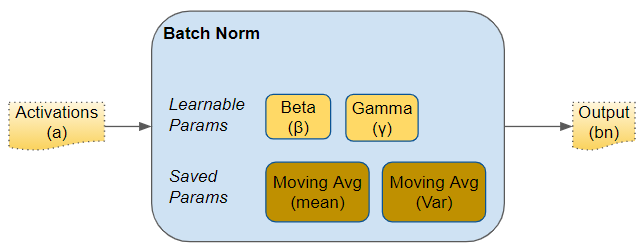
\includegraphics[width=1.0\textwidth,height=1.0\textheight,keepaspectratio]{images/BatchNorm1.png}
    \end{figure}
    %\footnotetext{\href{https://towardsdatascience.com/batch-norm-explained-visually-how-it-works-and-why-neural-networks-need-it-b18919692739/}{Ketan Doshi}}
\end{frame}

\begin{frame}{Batch Normalization}
\begin{figure}
\centering
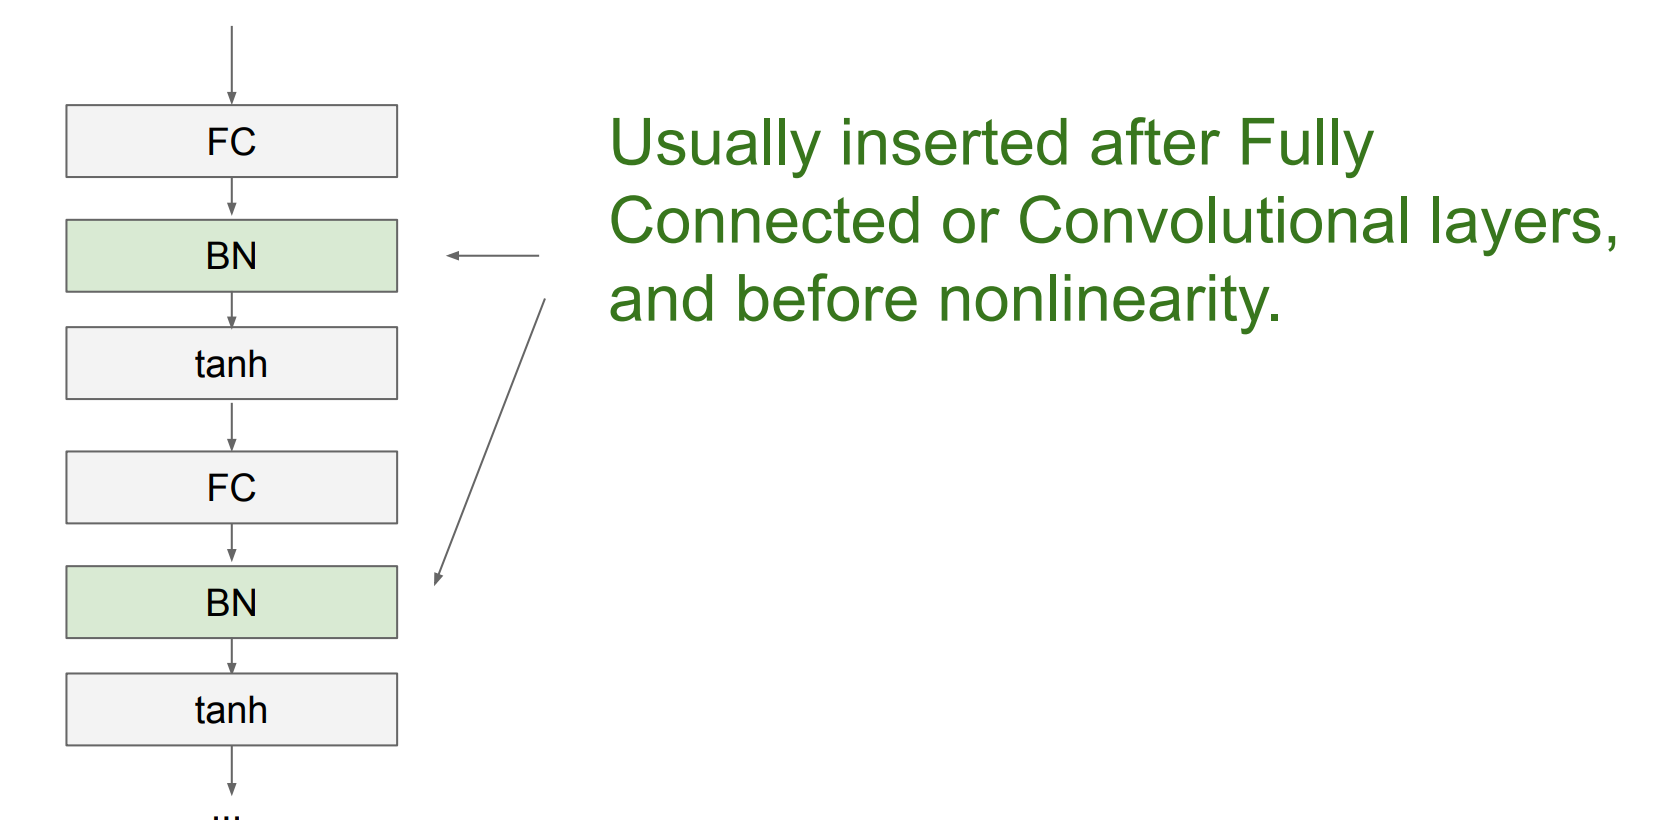
\includegraphics[width=1.0\textwidth,height=0.9\textheight,keepaspectratio]{images/bn4.png}
\end{figure}
% \footnotetext{\href{https://towardsdatascience.com/batch-norm-explained-visually-how-it-works-and-why-neural-networks-need-it-b18919692739/}{Ioffe and Szegedy 2015}}
\end{frame}

\begin{frame}{Batch Normalization}
    \begin{itemize}
        \item In Pytorch, batch normalization behavior is controlled by model's mode:
            \begin{block}{}
        \texttt{\small
        \# Training Mode: Use batch statistics\\
        model.train() \\
        output = model(input) \\
        \\
        \# Evaluation Mode: Use running statistics\\
        model.eval() \\
         output = model(input)
        }
    \end{block}
    \end{itemize}
\end{frame}

\begin{frame}{Batch Normalization}
\begin{itemize}
    \item Advantages:
    \begin{itemize}
        \item Makes deep networks much easier to train!
        \item Improves gradient flow
        \item Allows higher learning rates, faster convergence
        \item Networks become more robust to initialization
        \item Acts as regularization during training
        \item Zero overhead at test-time: can be fused with conv!
    \end{itemize}
    \pause
    \item Disadvantages:
    \begin{itemize}
        \item Behaves differently during training and testing: this is a very common source of bugs!
    \end{itemize}
\end{itemize}
% \footnotetext{Slide based on CS231n by Fei-Fei Li, Yunzhu Li \& Ruohan Gao}
\end{frame}

\begin{frame}{Batch Normalization}
\begin{figure}
\centering
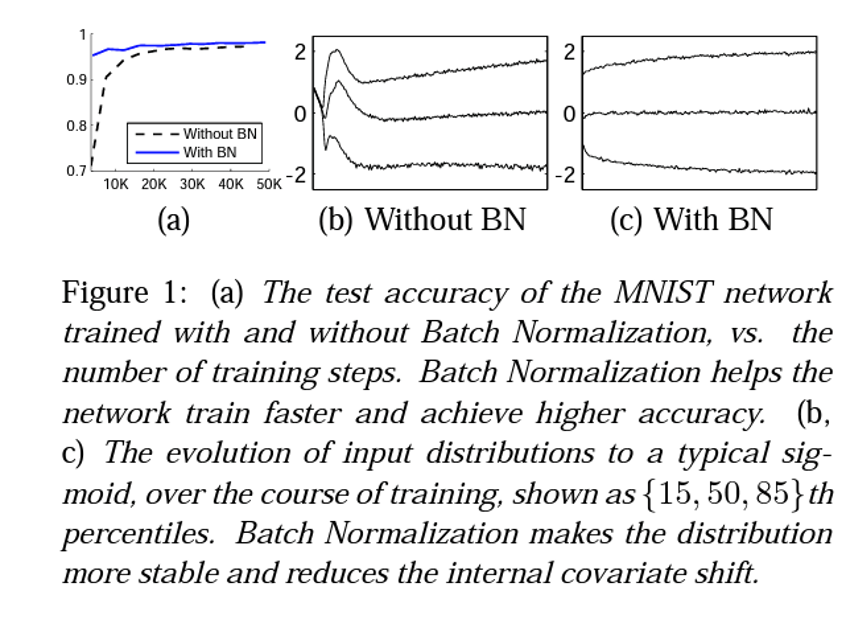
\includegraphics[width=1.0\textwidth,height=0.9\textheight,keepaspectratio]{images/batch_norm_6.png}
\end{figure}
% \footnotetext{\href{https://arxiv.org/pdf/1502.03167v3.pdf}{Ioffe and Szegedy 2015}}
\end{frame} 